\section{Send and Wait}

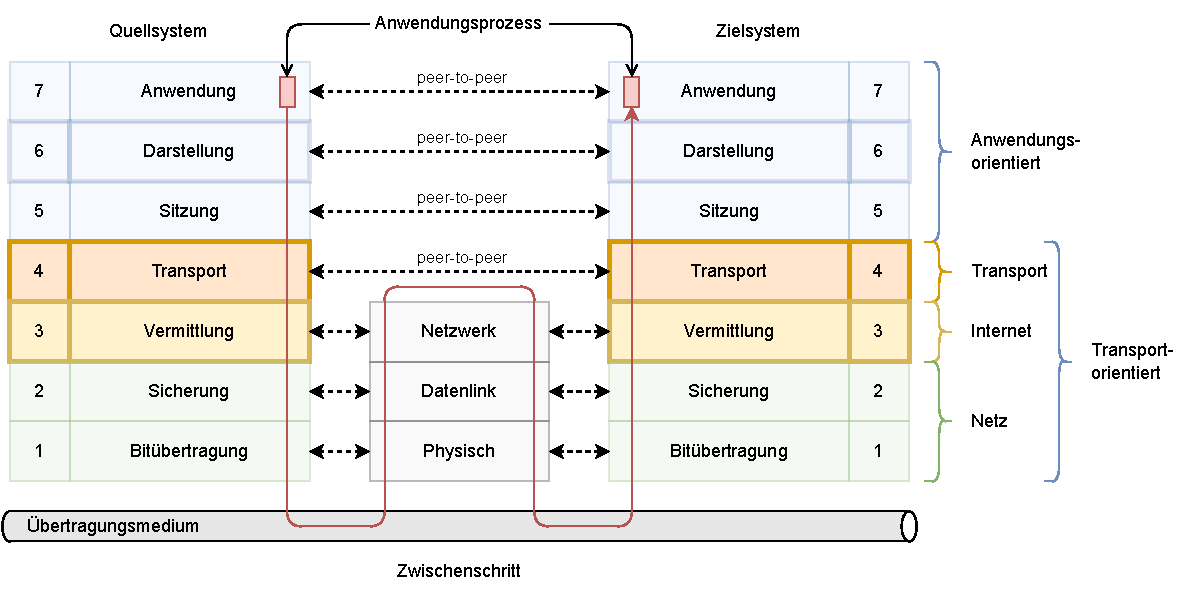
\includegraphics[width=\textwidth]{includes/figures/defi_iso_osi_transport_und_vermittlung.pdf}

\begin{bonus}{Probleme unsicherer Datenkanäle}
    Bei unsicheren Übertragungskanälen (wie z. B. IP) können folgende Fehler auftreten:
    \begin{itemize}
        \item Pakete können verloren gehen
        \item Die Reihenfolge kann vertauscht werden
        \item Pakete können Fehlerhaft empfangen werden
    \end{itemize}
\end{bonus}

\begin{bonus}{Zuverlässige Transportprotokolle}
    Wir wollen einen kontinuierlichen Datenstrom in Nachrichteneinheiten (Segmente) unterteilen, die eindeutig identifizierbar sind und im Anschluss sicher versenden.
    Wir können davon ausgehen, dass sich die beiden Geräte bereits kennen und eine Verbindung aufgebaut haben.

    Erforderliche Mechanismen:
    \begin{itemize}
        \item Fehlererkennung und ggf. -behebung
              \begin{itemize}
                  \item Der Empfänger muss Bitfehler in der Übertragungskanälen erkennen
                  \item Der Empfänger muss das Fehlen eines Segmentes erkennen und darauf reagieren (Obacht: Pakete können sich ebenfalls nur verspäten).
              \end{itemize}
        \item Empfänger-Feedback
              \begin{itemize}
                  \item Quittierungsnachrichten zwischen Empfänger und Sender
                  \item \emph{positive Acknowledgment} (\texttt{ACK}), welches den korrekten Erhalt bestätigt
                  \item Optional: \emph{negative Acknowledgment} (\texttt{NAK}), welches den Sender über Lücken oder Fehler informiert
              \end{itemize}
        \item Neuübertragung:
              \begin{itemize}
                  \item Sender überträgt Fehlerhafte Segmente erneut
                  \item Timer- bzw. \texttt{NAK}-gesteuert
              \end{itemize}
    \end{itemize}
\end{bonus}

\begin{defi}{ARQ-Protokoll}
    Das \emph{Automatic-Repeat-Request-Protokoll (ARQ)}, auch \emph{Send and Wait-Protokoll}, besteht daraus, dass Empfänger Bestätigungen (\texttt{ACK}s) bei korrektem Empfang versenden.

    Fehlerhafte Übertragungen werden durch Ausbleiben der Bestätigung erkannt und durch wiederholtes Versenden behoben.
\end{defi}

\begin{defi}{Einfaches ARQ-Protokoll}
    Der Sender geht segmentweise vor.
    Beim Senden startet er einen Timer zur Fehleridentifikation.
    Bei Erhalt des \texttt{ACK} wird das nächste Paket gesendet.
    Sobald nach Ablaufen des Timers noch kein \texttt{ACK} empfangen wurde, wird die Übertragung wiederholt.

    \begin{center}
        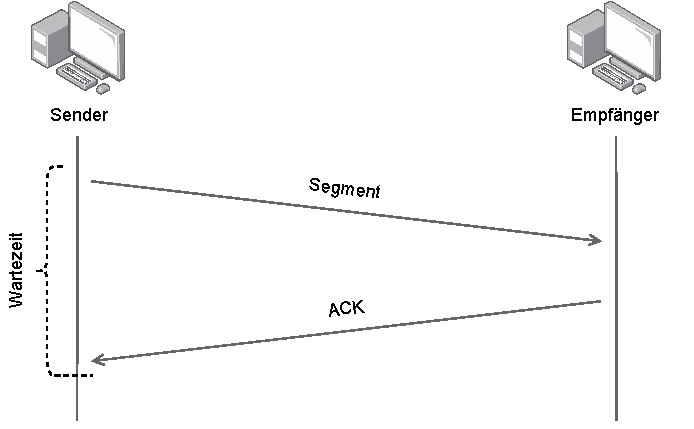
\includegraphics[width=0.75\textwidth]{includes/figures/defi_arq.pdf}
    \end{center}

    Der Datenstrom ist begrenzt auf ein Paket pro Zyklus.

    Sei die Länge eines Segments (L) in bits und die Übertragungsrate eines Kanals in $\nicefrac{\text{bits}}{s}$ gegeben, so wird die genutzte Übertragungszeit mit $\nicefrac{L}{R}$ errechnet.

    Die Wartezeit bzw. der Timeout (RTT) ist durch die genutzte Übertragungsart in Sekunden gegeben.

    Der Nutzungsgrad $\rho$ wird wie folgt berechnet:
    \[
        \rho := \frac{\text{genutze Übertragungszeit}}{\text{genutze Übertragungszeit} + \text{Wartezeit}} = \frac{\frac{L}{R}}{\frac{L}{R} + RTT}
    \]
\end{defi}

\begin{example}{Einfaches ARQ-Protokoll}
    \begin{center}
        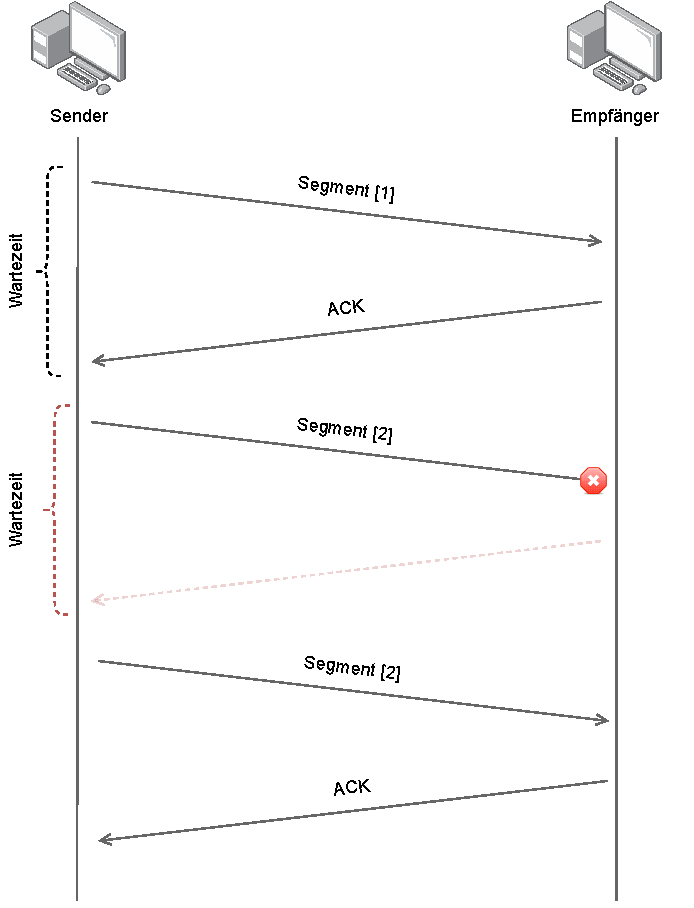
\includegraphics[width=0.5\textwidth]{includes/figures/example_arq.pdf}
    \end{center}
\end{example}

\begin{bonus}{Verfahren bei Fehler- bzw. Sonderfällen}
    \begin{center}
        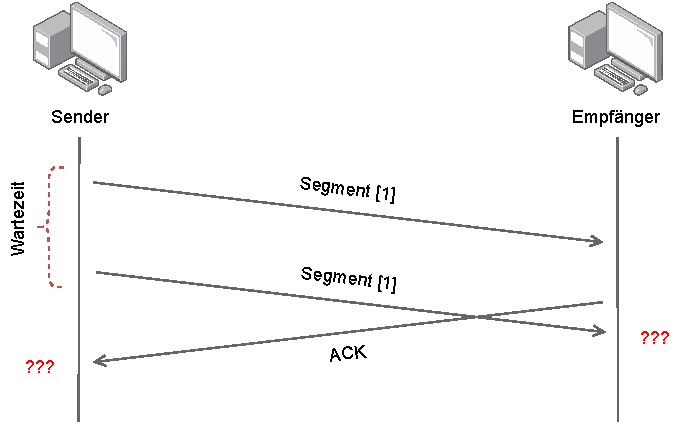
\includegraphics[width=0.5\textwidth]{includes/figures/bonus_arq_error.pdf}
    \end{center}

    Wenn wir länger als erwartet brauchen um das Paket zu versenden, wird immer vor Erhalt der Bestätigung neu versendet.
    Der Empfänger weiß nicht, welches Segment empfangen wurde und der Sender weiß nicht, für welches Paket er eine Bestätigung erhalten hat.

    Um das Problem zu lösen versehen wir jedes Paket mit einer eindeutigen ID.
    Diese entspricht entweder dem 1. Byte der Nachricht oder wird zyklisch durchnummeriert:

    \begin{center}
        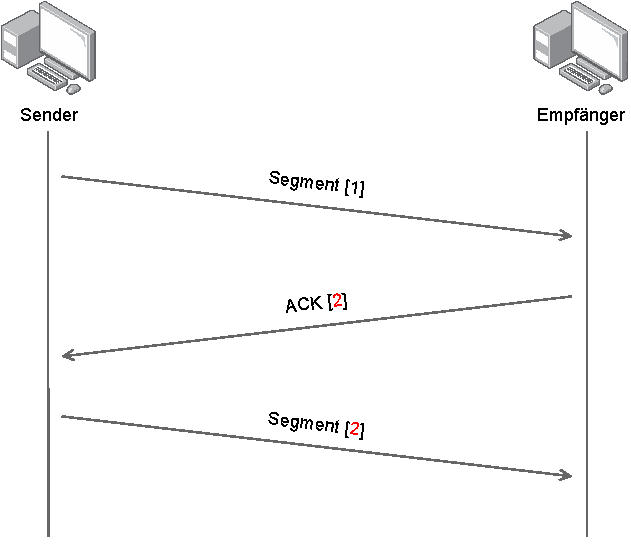
\includegraphics[width=0.5\textwidth]{includes/figures/bonus_arq.pdf}
    \end{center}
\end{bonus}

\begin{defi}{Pipelining}
    Um das Netz besser auszulasten nutzt man \emph{Pipelining}:
    \begin{itemize}
        \item Senden weiterer Segmente ohne vorheriges \texttt{ACK}
        \item Die Fensterbreite beim Sender richtet sich nach der Anzahl der Segmente, die ohne Bestätigung gesendet werden.
        \item Die Fensterbreite beim Empfänger richtet sich nach der Anzahl der Segmente, die auch bei Lücken oder Fehlern zwischengespeichert werden.
    \end{itemize}

    Sei $n$ die Fensterbreite des Senders.
    Dann wird der Nutzungsgrad $\rho$ wie folgt berechnet:
    \[
        \rho := n \cdot \frac{\frac{L}{R}}{\frac{L}{R} + RTT}
    \]
\end{defi}

\begin{example}{Pipelining}
    \begin{center}
        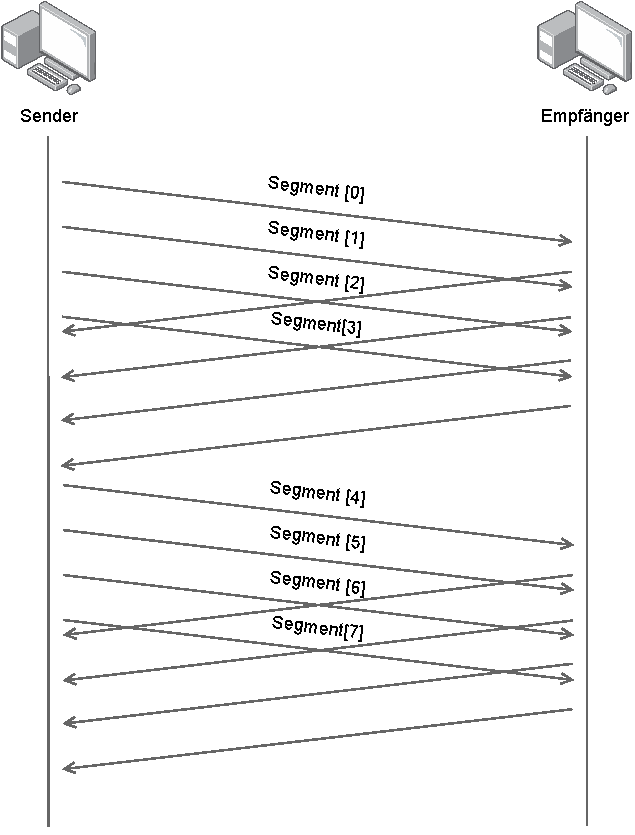
\includegraphics[width=0.5\textwidth]{includes/figures/example_pipelining.pdf}
    \end{center}
\end{example}

\begin{defi}{Go-Back-N}
    \emph{Go-Back-N} ist ein Verfahren um nach Fehlern das Senden sinnvoll fortzusetzen.

    Sobald der Sender kein \texttt{ACK} erhält, läuft er in einen Timeout (Fensterbreite) und springt danach hinter das Paket, welches als letztes erfolgreich versendet wurde.

    Alle direkt nach dem Fehler versendeten Segmente werden verworfen.
\end{defi}

\begin{example}{Go-Back-N}
    \begin{center}
        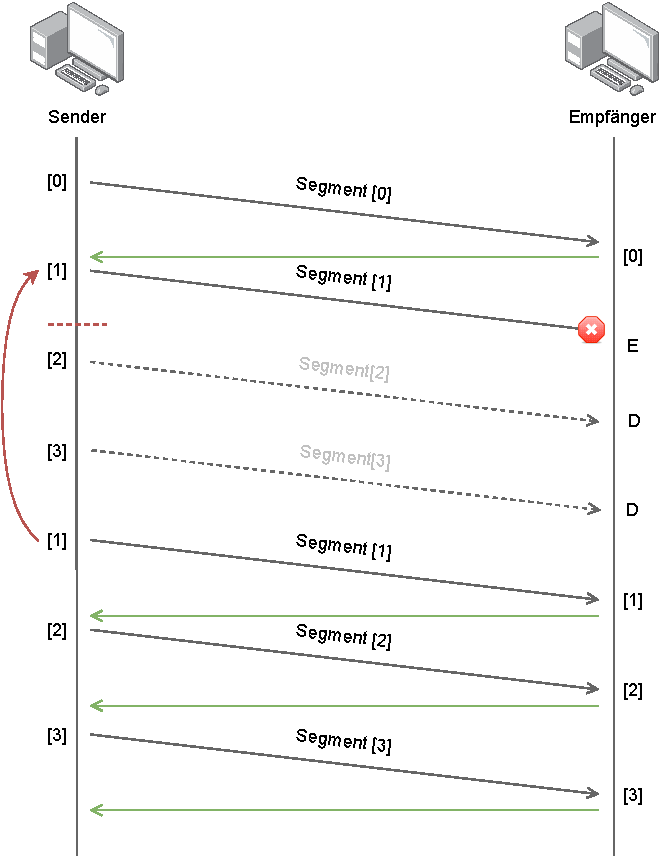
\includegraphics[width=0.5\textwidth]{includes/figures/example_go_back_n.pdf}
    \end{center}

    Der Client sendet kein \texttt{ACK} auf Fehler (\texttt{E}) und verwirft Frames, die unerwartet empfangen werden (\texttt{D}).
\end{example}